\subsection{User Journeys}

\subsubsection{Client Journey}

\bigskip

\begin{figure}[H]
    \centering
    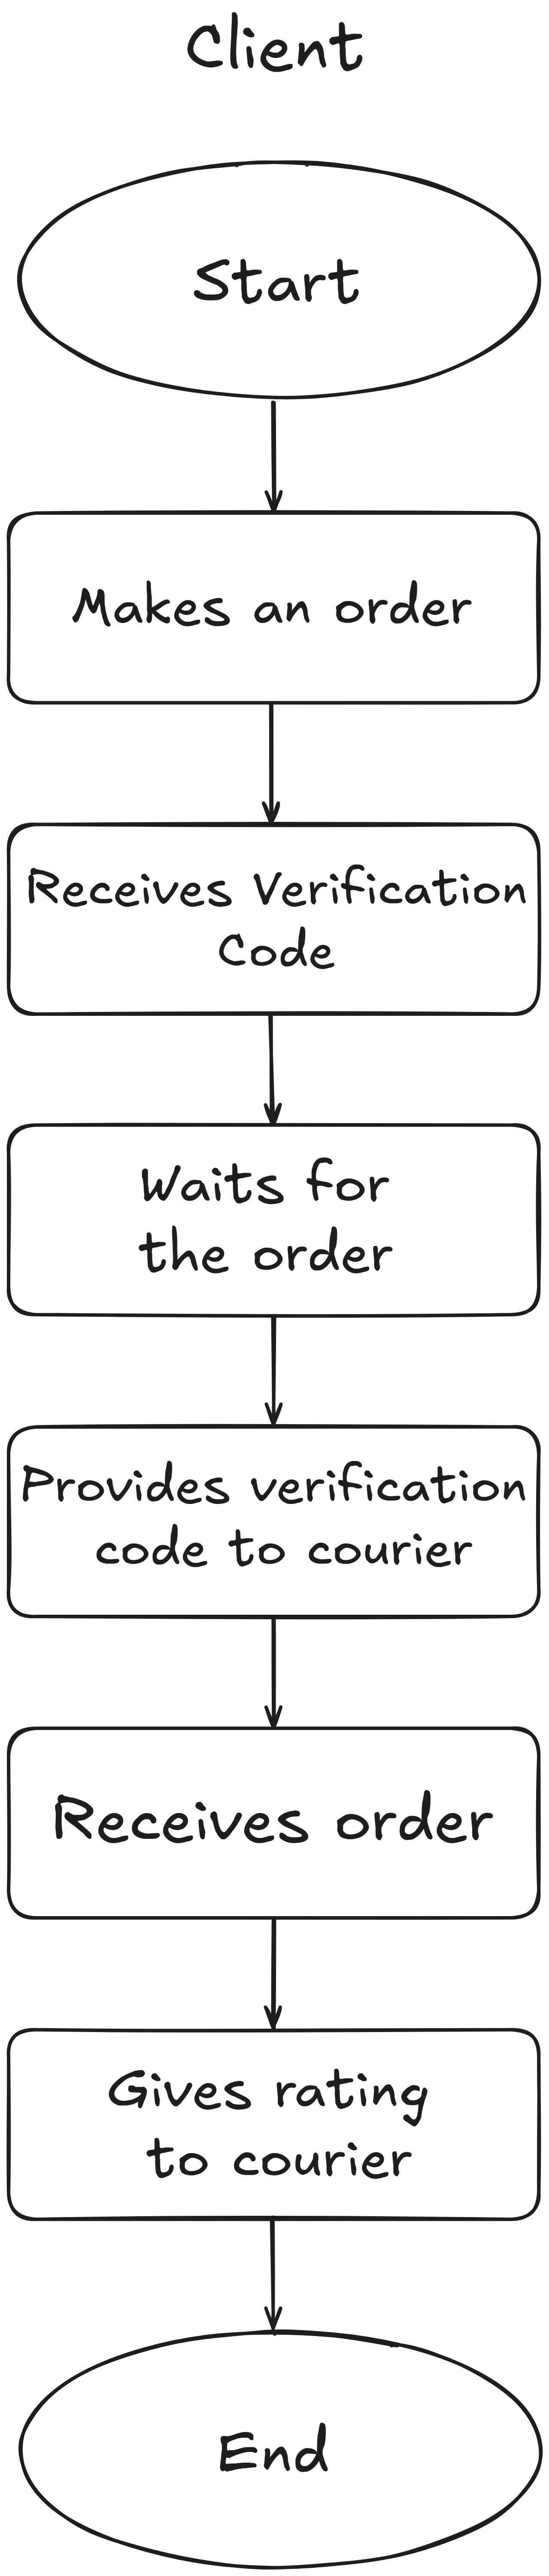
\includegraphics[width=0.2\textwidth]{images/ClientJourney.png} % adjust path & width if needed
    \caption{Client journey flowchart showing from the beginning}
    \label{fig:client_journey}
\end{figure}

This flowchart (\ref{fig:client_journey}) illustrates the sequential steps a client undergoes when placing an order through the LiftDrop platform. The process begins with the client initiating an order, followed by a waiting period for the order to be processed and accepted by a courier. Once the order is received, the client provides a unique confirmation code to the courier, marking a secure handoff. Finally, the process concludes with the client rating the delivery experience.

\newpage

\subsubsection{Courier Journey}

\bigskip

\begin{figure}[H]
    \centering
    \includegraphics[width=0.37\textwidth]{images/CourierJourney.png} % adjust path & width if needed
    \caption{Courier journey flowchart showing from the beginning}
    \label{fig:courier_journey}
\end{figure}

This flowchart (\ref{fig:courier_journey}) outlines the step-by-step decision-making process a courier follows while managing delivery requests on the LiftDrop platform. It begins with the courier awaiting an incoming order, which can either be accepted or rejected. Upon accepting a request, the courier proceeds to the pickup location, with the option to cancel if necessary. After pickup, the courier advances to the delivery phase. If the courier successfully reaches the destination, the delivery is confirmed. If the destination is not reached, the system prompts reevaluation or cancellation.

\newpage